\section{Neuro-Adaptive Control}

\subsection{What is Neuro-Adaptive Control?}

\begin{frame}{\insertsubsectionhead}
  
  \textbf{Neuro-Adaptive Control}
  \small{
    \begin{itemize}
      \item \textbf{Neuro-adaptive control} (NAC) is a control strategy that combines \ctxt{airforceblue}{neural networks (NNs) } with \ctxt{awesome}{adaptive control } \cite{Farrell:2006aa}.
      \item Features of both \ctxt{airforceblue}{NNs } and \ctxt{awesome}{adaptive control } can be found in NAC.
    \end{itemize}
  }

  \begin{figure}
    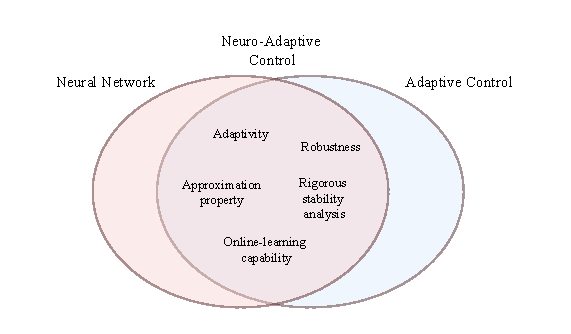
\includegraphics[width=0.65\textwidth]{figures/NAC.drawio.pdf}
  \end{figure}

\end{frame}

\begin{frame}{\insertsubsectionhead}

  \textbf{Advantages of Neuro-Adaptive Control}
  \small{
    \begin{itemize}
      \item <2-> \textbf{Adaptability}: NAC adapts \ctxt{airforceblue}{NN weights }to changing environments and system dynamics.
      \item <3-> \textbf{Stability Guarantee}: The closed-loop stability is ensured using \ctxt{airforceblue}{Lyapunov stability theory}.
      \item <4-> \textbf{Online Learning Capability}: NAC adapts in \ctxt{airforceblue}{real-time } to new data with stability guarantees.
      \item <5-> \textbf{Robustness}: NAC handles \ctxt{airforceblue}{uncertainties and disturbances }effectively with adaptive control techniques.
    \end{itemize}
  }
  
\begin{figure}
  \label{fig:general_framework}
  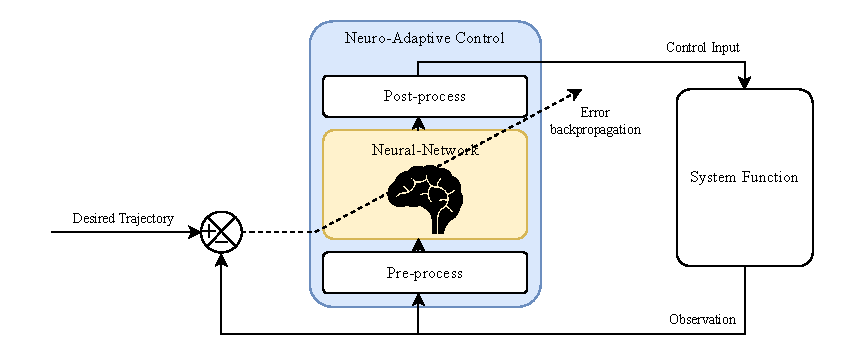
\includegraphics[width=0.65\textwidth]{figures/conv_nac.drawio.pdf}
  \caption{General framework of neuro-adaptive control (NAC).}
\end{figure}

\end{frame}

\subsection{Existing Challenges in NAC}

\begin{frame}{\insertsubsectionhead}

%   \textbf{Existing Challenges in NAC}

  \begin{enumerate}
    
    \onslide<1->
    {
      \begin{columns}[T,onlytextwidth]

        \column{0.49\textwidth}

          \small{
            \item \textbf{Weight Boundedness:} 

            \begin{itemize}
              \item Generally, NN weights are adapted by \ctxt{airforceblue}{gradient descent method}.
              \begin{itemize}
                \item Objective function typically consists of the control error.
              \end{itemize}
              \item Hence, the NN weights can grow \ctxt{awesome}{unbounded}, leading to instability (also known as \textit{parameter drift}).
              \item Unbounded weights can cause the NN to produce \ctxt{airforceblue}{large control inputs}, which may lead to following challenges.
            \end{itemize}
          }
            
          \column{0.49\textwidth}
            \centering

              \begin{figure}
                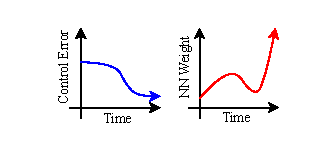
\includegraphics[width=0.7\textwidth]{figures/unbounded.drawio.pdf}
                \caption{Divergence of NN weights even with convergent control error.}
              \end{figure}
        \end{columns}
      }

      \onslide<2->
      {
        \begin{columns}[T,onlytextwidth]
          \column{0.49\textwidth}

          \small{
            \item \textbf{Control Saturation} \textit{(unpredictable amplitude of NN outputs)}: 

            \begin{itemize}
              \item Typical issue of control problem in physical systems.
              \item The NN outputs are \ctxt{awesome}{unpredictable } and \ctxt{awesome}{not interpretable}.
              \item These features—unbounded NN weights and unpredictable amplitudes—can lead to \ctxt{airforceblue}{input saturation}.
            \end{itemize}
          }

          \column{0.49\textwidth}
            \centering
            \begin{figure}
              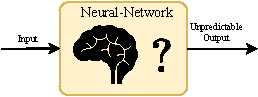
\includegraphics[width=0.8\textwidth]{figures/unpredictable.drawio.pdf}
              \caption{Unpredictable amplitude of NN outputs.}
            \end{figure}
        \end{columns}
      }

  \end{enumerate}

\end{frame}

\subsection{Proposed Method: Constrained Optimization-Based NAC (CONAC)}

\begin{frame}{\insertsubsectionhead}
  
  \begin{columns}
    
    \column{0.5\textwidth}
      
    \onslide<2->
    {
      \textbf{Target System}:
      \small{
        \begin{itemize}
          \item Control input \ctxt{awesome}{saturation function } $\mysat(\cdot)$.
          \item Desired trajectory $\mv{x}_d$ is given.
        \end{itemize}
          \begin{equation}\label{eq:sys}
            \ddtt \mv{x} 
            =
            \mv{f}(\mv{x})
            +
            \mv{g}(\mv{x})
            \mysat(\mv{u})
          \end{equation}    
      }
    }
    
    \onslide<3->
    {
      \textbf{Control Input}:
      \small{
        \begin{itemize}
          \item NN's \ctxt{airforceblue}{output } $\mv{\Phi}$ is used as the control input.
          \item Consists of the \ctxt{awesome}{estimated NN weights } $\estwth$.
        \end{itemize}
        \begin{equation}\label{eq:input}
          \mv{\mv{u}} := \mv{\Phi}(\mv{q}_n; \estwth)
        \end{equation}
      }
    }

    \onslide<4->
    {
      \textbf{Deep Neural Network (DNN)}:
      \small{
        \begin{itemize}
          \item $k$ layers with weights $\estwth_i:=\myvec(\estwV_i)$.
          \item Activation function: $\phi(\cdot):=tanh(\cdot)$.
          \begin{equation}\label{eq:NN}
            \mv{\Phi}(\mv{q}_n; \estwth)
            :=
            \begin{cases}
                \estwV_i^\top \act_i(\estNN_{i-1}), 
                &
                i\in\{1,\dots ,k\},
                \\
                \estwV_0^\top {\q}_n,
                &
                i=0
                ,
            \end{cases}
          \end{equation}
        \end{itemize}
      }
    }

    \column{0.5\textwidth}  

    \onslide<4->
    {
      \begin{figure}
        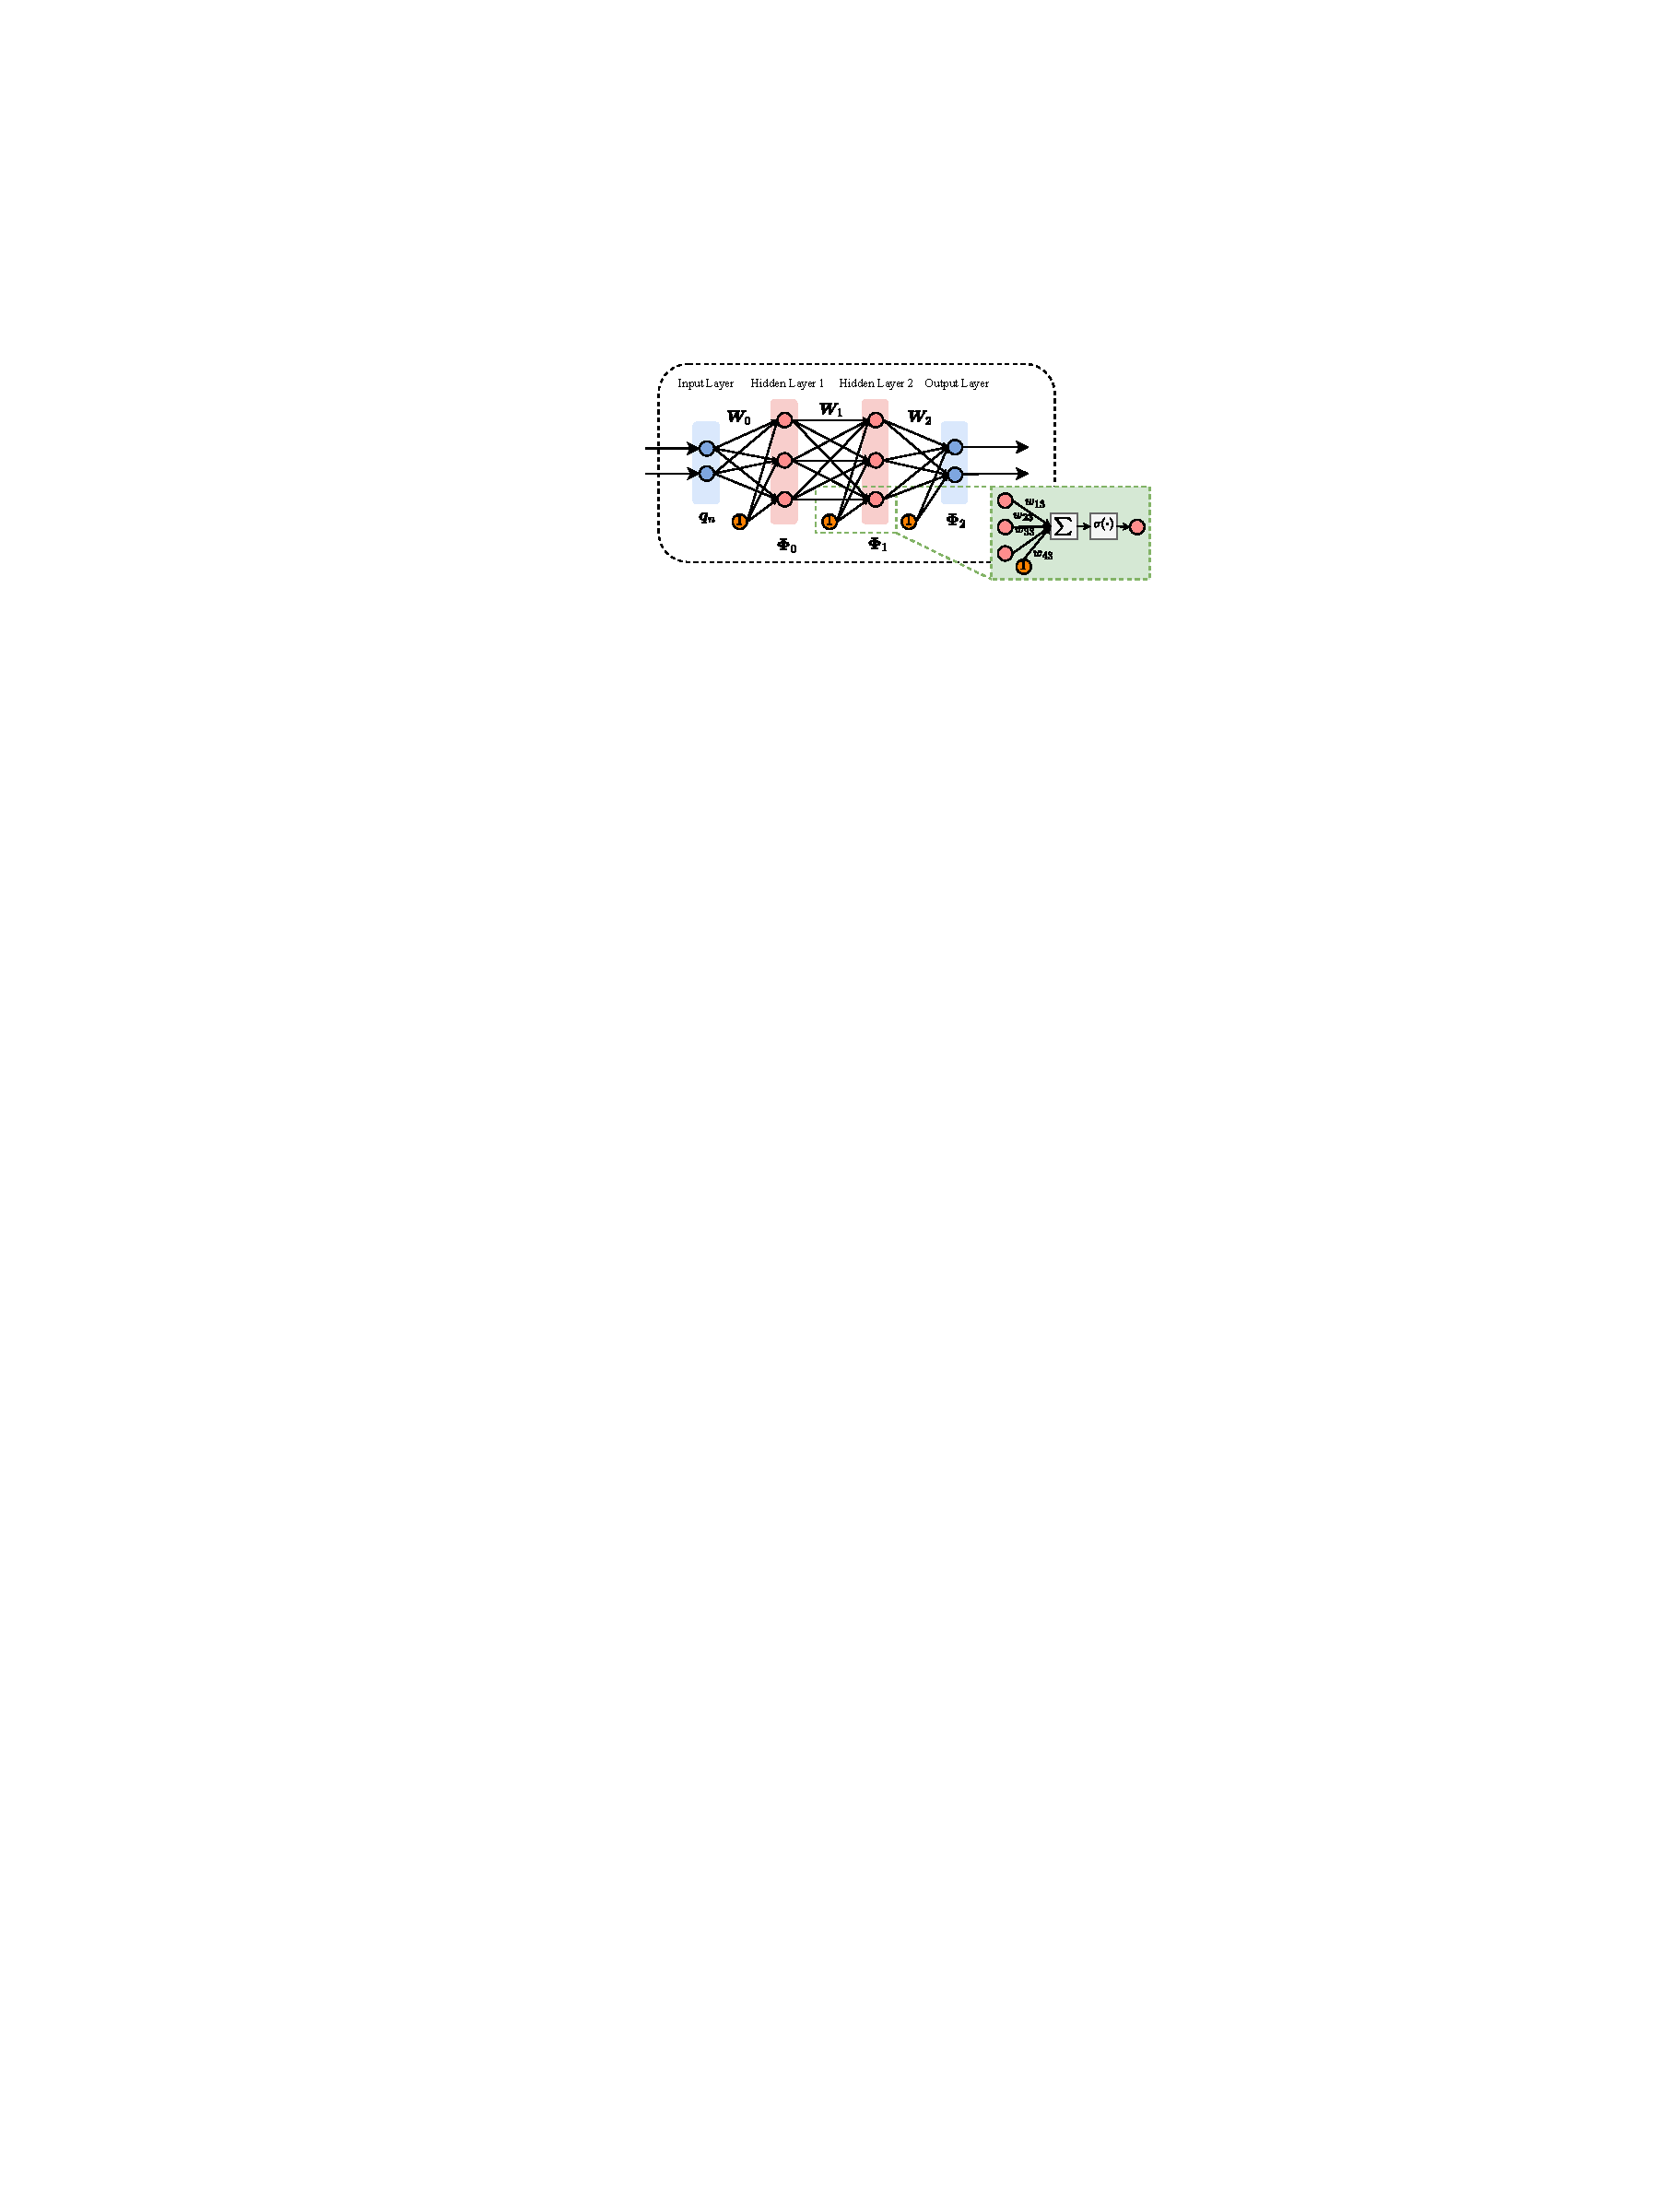
\includegraphics[width=0.7\textwidth]{figures/DNN.drawio.pdf}
        \caption{Architecture of the DNN.}
      \end{figure}
    }

  \end{columns}

    \let\thefootnote\relax\footnote{
      \textit{Notations}: 
        $\mv{q}\in\R^n$: Joint position, $\mm{M}$: Inertia matrix, $\mm{C}$: Coriolis matrix, $\mm{G}$: Gravity vector, $\mv{\tau}$: Control input, $\mv{\tau}_d$: Disturbance.
      }

\end{frame}

\begin{frame}{\insertsubsectionhead}{}

\begin{columns}

  \column{0.45\textwidth}

    \textbf{Optimization Problem Statement}:

    \begin{itemize}
      \item \ctxt{awesome}{Find } NN weights $\estwth$,
      \item That \ctxt{airforceblue}{minimize } objective function $J(\cdot)$,
        \begin{equation}\label{eq:obj}
          J(\mv{e};\estwth)
          := 
          \frac{1}{2} \mv{e}^\top \mv{e}.
        \end{equation}
        \begin{itemize}
          \item where $\mv{e} := \mv{x} - \mv{x}_d$ is \ctxt{awesome}{tracking error},
        \end{itemize}
      \item while satisfying the following \ctxt{awesome}{constraints}:
        \begin{itemize}
          \item \ctxt{airforceblue}{Boundedness } of the NN weights $\estwth$.
          \item \ctxt{airforceblue}{Saturation } of the control input $\mv{u}$.
        \end{itemize}
    \end{itemize}

  
  \column{0.5\textwidth}

  \onslide<2->
  {
    \begin{block}{Considered Constraints}

      \begin{itemize}
        \item \textbf{Weight Boundedness for Each Layer}: 
          \begin{equation}\label{eq:cstr:weight}
            c_{\theta_i}(\estwth)
            :=
            \norm{\estwth_i}^2 - \overline{\theta_i}^2 \le 0
            , 
            \forall i\in\{0,\ldots,k\}
          \end{equation}

        \item \textbf{Convex control Input Saturation}: 
          \begin{itemize}
            \item Input bound constraint \textit{for each control input}:
            \begin{equation}\label{eq:cstr:input_bound}
              c_{\overline{u}_i}(\estwth)
              :=
              u_i - \overline{u_i}
              \le 
              0
              ,
              \quad
              c_{\underline{u}_i}(\estwth)
              :=
              \underline{u_i} - u_i
              \le 
              0
            \end{equation}
            \item Input norm constraint:
            \begin{equation}\label{eq:cstr:input_norm}
              c_{\mv{u}}(\estwth)
              :=
              \norm{\mv{u}}^2 - \overline{u}^2
              \le
              0
            \end{equation}
        \end{itemize}
      \end{itemize}
      
    \end{block}
  }

  \end{columns}

\end{frame}

%~~~~~~~~~~~~~~~~~~~~~~~~~~~~~~~~~~~~~~~~~~~~~~~~~~~~~~~~~~~~~~~~~~~~~~~~~~~~~~
\begin{frame}{\insertsubsectionhead}{}
  
  To solve the dual problem from constrained optimization theory,
  \begin{equation}
    \min_{\estwth}\max_{[\lambda_j]_{j\in\mathcal{I}}} 
    L(\mv{r},\estwth,[\lambda_j]_{j\in\mathcal{I}})
    =
    \min_{\estwth}\max_{[\lambda_j]_{j\in\mathcal{I}}}
    \left(
        J(\mv{e};\estwth)
        +
        \textstyle\sum_{j\in\mathcal{I}}
        \lambda_j c_j(\estwth)
    \right)
    ,
  \end{equation}
  the first-order gradient descent/ascent method is used to derive the adaptation law.

  \centering
  \begin{minipage}{0.6\textwidth}%

    \begin{block}{Adaptation Law}%
      
    \onslide<2->
    {
      \textbf{Gradient \ctxt{airforceblue}{Descent } Method for weights $\estwth$}:
      \begin{equation}\label{eq:adaptation_law:1}
        \ddtt {
          \ctxt{airforceblue}{\estwth}
          }
        =
        -\alpha 
        \pptfrac{L}{\ctxt{airforceblue}{\estwth}}
        =-\alpha 
        \left(
            \pptfrac{J}{\ctxt{airforceblue}{\estwth}}
            +
            \textstyle\sum_{j\in\mathcal{I}}
            \ctxt{awesome}{\lambda_j}
            \pptfrac{c_j}{\ctxt{airforceblue}{\estwth}}
        \right),
      \end{equation}
    }

    \onslide<3->
    {
      \textbf{Gradient \ctxt{awesome}{Ascent } Method for Lagrange multipliers $\lambda_j, \forall j\in\mathcal I$}:
      \begin{equation}\label{eq:adaptation_law:2}
        \ddtt\ctxt{awesome}{\lambda_j}
        = 
        \beta_j
        \pptfrac{L}{\ctxt{awesome}{\lambda_j}} 
        = 
        \beta_j c_j ,
      \end{equation}
    }

    \onslide<4->
    {
      For non-negativity of the Lagrange multipliers,
      \begin{equation}\label{eq:adaptation_law:3}
        \ctxt{awesome}{\lambda_j}
        \leftarrow
        \max(\ctxt{awesome}{\lambda_j},0)
        .
      \end{equation}
    }

    \end{block}
  \end{minipage}
  
  \let\thefootnote\relax\footnote{
    $\alpha$: adaptation gain (learning rate), $\beta_j$: update rate of the Lagrange multipliers.
  }

\end{frame}

\begin{frame}{\insertsubsectionhead}{}

    \textbf{Stability Guarantee using Lyapunov Theory}

  \centering
  \begin{minipage}{.9\textwidth}

    \begin{block}{Theorem 1 \cite{Ryu:2025aa}}
      For the \ctxt{airforceblue}{dynamical system }, the \ctxt{awesome}{neuro-adaptive controller } with the \ctxt{airforceblue}{weight adaptation laws } in \eqref{eq:adaptation_law:1}, \eqref{eq:adaptation_law:2} and \eqref{eq:adaptation_law:3} ensure the \ctxt{airforceblue}{boundedness } of the \ctxt{awesome}{filtered error } $\mv{r}$ and the \ctxt{awesome}{weight estimate } $\estwth$, under the \ctxt{airforceblue}{control input constraints} satisfying Assumption 1 and 2. This holds under the \ctxt{awesome}{weight norm constraint } \eqref{eq:cstr:weight}.
    \end{block}

    \begin{exampleblock}{Assumption 1 (Convex Input Constraint)}
      The constraint functions $c_j(\estwth),\forall j\in\mathcal{I}$, are convex in the $\tau$-space and satisfy $c_j(\estwth)\le0$ and $c_j(\idealwth)\le0$.
    \end{exampleblock}

    \begin{exampleblock}{Assumption 2, Linear Independence Constraint Qualification (LICQ)}
      The selected constraints satisfy the Linear Independence Constraint Qualification (LICQ) \cite[Chap. 12 Def. 12.1]{Nocedal:2006aa}.
    \end{exampleblock}

  \end{minipage}

  \vspace{.2cm}

  Proof of Theorem 1 is \textbf{omitted } due to space limitations. The detailed proof can be found in \cite{Ryu:2025aa}.

\end{frame}

\subsection{Demonstration Video}

\begin{frame}{\insertsubsectionhead}

  \begin{itemize}
    \item This video demonstrates:
    \begin{itemize}
      \item \ctxt{airforceblue}{Applicability }of the proposed method to real-time control (under 4 ms sampling time).
      \item \ctxt{awesome}{Convex input constraints } handling.
    \end{itemize}
  \end{itemize}

  \centering
  \includemedia[
      width=0.64\linewidth,
      height=0.36\linewidth,
      activate=onclick,
      addresource=assets/animationECC.mp4,
      flashvars={
        source=assets/animationECC.mp4
        &autoPlay=true
        &loop=true
      }
    ]{}{VPlayer.swf}

\end{frame}

\subsection{Summary}

\begin{frame}{\insertsubsectionhead}

    \textbf{Summary of Contributions}

  \begin{itemize}
    \item \cblue{Constraints} (weight and input) are imposed in \cred{adaptation law derivation} for NAC using \cblue{constrained optimization theory}.
    \item \cred{Stability guarantee} of the proposed method is provided using \cblue{Lyapunov theory}.
    \item \cblue{Real-time feasibility} of the proposed method is demonstrated through a video of a real-time control experiment.
  \end{itemize}

  \hfill

  \textbf{Related published papers} can be found in 
  \begin{enumerate}
    \item
        Imposing a Weight Norm Constraint for Neuro-Adaptive Control, \cblue{European Control Conference (ECC)}, pp. 380-385, 2025
    \begin{itemize}
        \item \cred{\textit{Weight Norm Constraint for NAC}}
    \end{itemize}
    \item
        Constrained Optimization-Based Neuro-Adaptive Control (CONAC) for Synchronous Machine Drives Under Voltage Constraints, \cblue{Annual Conference of the IEEE Industrial Electronics Society (IECON)}, pp. 1-7, 2025
    \begin{itemize}
        \item \cred{\textit{Input Norm Constraint for VSI in NAC on SM Drives}}
    \end{itemize}
    \item
        Constrained Optimization-Based Neuro-Adaptive Control (CONAC) for Euler-Lagrange Systems Under Weight and Input Constraints, \cblue{Under Review}, 2026
    \begin{itemize}
        \item \cred{\textit{Weight and Convex Input Constraints for NAC}}
    \end{itemize}
  \end{enumerate}

\end{frame}